\chapter{Inversione della cinematica differenziale}
\paragraph{}
L'equazione cinematica differenziale, rappresenta una trasformazione lineare tra \emph{spazio dei giunti} e \emph{spazio operativo}, infatti, essa stabilisce un legame lineare tra le \emph{velocità ai giunti} e la \emph{velocità dell'organo terminale} anche se è dipendente dalla \emph{configurazione del manipolatore}. Quindi, possiamo utilizzare l'equazione cinematica differenziale per affrontare il problema dell'inversione cinematica.  
\paragraph{}
Si supponga assegnata per l'organo terminale una \emph{traiettoria di moto} specificando $\underline{v}_{\,des}(t)$ e le condizioni iniziali su \emph{posizione e orientazione}. L'obiettivo è quello di determinare una possibile \emph{traiettoria ai giunti} $(\underline{q}(t), \underline{\dot{q}}(t))$ che riproduca la traiettoria data. Considerando la ($4.32$) nell'ipotesi $n = r$, ovvero, non vi sono manipolatori ridondanti e singolarità, otteniamo banalmente:
\begin{equation}
	\underline{\dot{q}} = J^{-1}(\underline{q})\,\underline{v}_{\,des}
\end{equation}
e chiaramente, conoscendo la postura iniziale del manipolatore $\underline{q}(0)$ possiamo calcolare la posizione $\underline{q}(t)$ integrando nel dominio del tempo. Questa integrazione si può effettuare al calcolatore tramite metodi numerici come quello di Eulero,
\begin{equation}
	\underline{q}(t) = \int_{t_i}^{t_f} \underline{\dot{q}}(t) dt \quad \Leftrightarrow \quad \underline{q}(t_{k+1}) = \underline{q}(t_k) + \underline{\dot{q}}(t_k)\Delta t 
\end{equation}

con l'istante $t_{k+1}$ scritto come: $t_{k+1} = t_k + \Delta t$. Quanto detto finora è valido solo se lo Jacobiano è a \emph{rango pieno}.

\section{Gestione della ridondanza}
Nel caso in cui si hanno delle ridondanze ($r<n$) e $J$ "obesa", un possibile metodo di soluzione è quello di formulare il problema della ricerca di soluzioni in termini di un problema di ottimo vincolato. Notiamo che $J$ potrebbe essere \emph{full rank}.
\paragraph{}
Una volta assegnata la velocità dell'organo terminale $\underline{v}_{\,des}$ e lo Jacobiano del manipolatore $J$ (per una data configurazione $\underline{q}$), si vogliono trovare le soluzioni $\underline{\dot{q}}$ che soddisfino l'equazione lineare ($4.32$) e che minimizzino il funzionale di costo quadratico delle velocità
\begin{equation}
	g(\underline{\dot{q}}) = \frac{1}{2}\underline{\dot{q}}^{T}W\underline{\dot{q}}
\end{equation}

dove $W\in\mathbb{R}^{n \times n}$ è una \emph{matrice di peso} simmetrica e definita positiva.\\
Il problema può essere risolto con il \emph{metodo dei moltiplicatori di Lagrange}, attraverso il \emph{funzionale di costo modificato},
\begin{equation}
	g(\underline{\dot{q}}, \underline{\lambda}) = \frac{1}{2}\underline{\dot{q}}^{T}W\underline{\dot{q}} + \lambda^T(\underline{v}_{\,des} - J\underline{\dot{q}})
\end{equation}

dove $\lambda \in\mathbb{R}^{r \times 1}$ è un vettore incognito di moltiplicatori che permette di incorporare il vincolo ($4.32$) nel funzionale da minimizzare, la soluzione cercata deve soddisfare le condizioni:
\begin{equation}
	\frac{\partial g}{\partial \underline{\dot{q}}} = 0 \qquad \frac{\partial g}{\partial \underline{\lambda}} = 0
\end{equation}
Otteniamo,
\begin{equation*}
	\begin{cases}
		\frac{\partial g}{\partial \underline{\dot{q}}} = \underline{\dot{q}}^TW - \underline{\lambda}^TJ = 0^T \\
		\frac{\partial g}{\partial \underline{\lambda}} = (\underline{v}_{\,des}- J\underline{\dot{q}})^T = 0^T
	\end{cases}
	\quad \Rightarrow \quad 
	\begin{cases}
		\underline{\dot{q}}^T = \underline{\lambda}^T JW^{-1} \\
		\underline{v}_{\,des} = J\underline{\dot{q}} 
	\end{cases}
	\quad \Rightarrow \quad
	\begin{cases}
		\underline{\dot{q}} = W^{-1}J^T \underline{\lambda} \\
		\underline{v}_{\,des} = JW^{-1}J^T \underline{\lambda}
	\end{cases}
\end{equation*}
Se $J$ è a rango pieno, anche $JW^{-1}J^T$ lo è, in quanto $W > 0$ e quindi ricaviamo 
\begin{equation}
	\underline{\lambda} = (JW^{-1}J^T)\underline{v}_{\,des}
\end{equation}

possiamo sostituirlo nell'espressione $\underline{\dot{q}} = W^{-1}J^T \underline{\lambda}$ e trovare $\underline{\dot{q}}$:
\begin{equation}
	\underline{\dot{q}} = \underbrace{W^{-1}J^T(JW^{-1}J^T)^{-1}}_{\text{pseudo-inversa pesata di J}}\,\underline{v}_{\,des}
\end{equation}

\paragraph{}
La matrice $W^{-1}J^T(JW^{-1}J^T)^{-1}$ è una \emph{inversa destra} di $J$, infatti, se premoltiplico per $J$ otteniamo
\begin{equation}
	J\Bigl[ W^{-1}J^T(JW^{-1}J^T)^{-1} \Bigr] = I_{r \times r}
\end{equation}

si può verificare infatti che la ($5.7$) soddisfa il vincolo di cinematica differenziale dato dalla ($4.32$) moltiplicando ambo i membri della ($5.7$) per $J$. Otteniamo infatti, $\underline{v}_{\,des} = J\,\underline{\dot{q}}$, ovvero, la ($4.32$).

\paragraph{}
Come sappiamo, la \emph{pseudo-inversa} esiste per ogni matrice, ma se scegliamo come \emph{matrice di peso} la matrice identità e $J$ è a \emph{rango pieno}, ricaviamo una particolare pseudo-inversa di $J$ detta \emph{pseudo-inversa di Moore Penrose},
\begin{equation}
	W = I_{r \times r} \quad \Rightarrow \quad \underline{\dot{q}} = \underbrace{ J^T(JJ^T)^{-1}}_{= J^{+}}\,\underline{v}_{\,des}
\end{equation}

è molto importante capire che se $J$ non ha rango pieno, $J^{+}$ non ha la forma scritta sopra. Notiamo che la $\underline{\dot{q}}$ trovata nella ($5.9$) minimizza la ($5.3$) e lo scarto $\| \underline{v}_{\,des} - J \underline{\dot{q}} \|$.
\newpage

\subsection{Soddisfacimento di vincoli aggiuntivi}
Ricordiamo, come detto nel paragrafo ($4.4.1$) che se $\underline{\dot{q}}^*$ soddisfa il vincolo $\underline{v}_{\,des} = J\underline{\dot{q}}^*$ e $P$ è un \emph{proiettore} su $\mathcal{N}(J)$, allora anche la seguente $\underline{\dot{q}}$ soddisfa il vincolo,
\begin{equation}
	\underline{\dot{q}} = \underline{\dot{q}}^* + P\underline{\dot{q}}_{\,a} \quad \textit{con $\underline{\dot{q}}_{\,a}$ arbitrario}
\end{equation}
\paragraph{}
Supponiamo di aver calcolato $\underline{\dot{q}}_{\,a}$ a partire da un criterio aggiuntivo che vogliamo soddisfare, formuliamo un problema di ottimizzazione con vincolo:
\begin{equation}
	g(\underline{\dot{q}}, \underline{\lambda}) = \frac{1}{2}(\underline{\dot{q}} - \underline{\dot{q}}_{\,a})^T \underbrace{I_{n \times n}}_{= W}(\underline{\dot{q}} - \underline{\dot{q}}_{\,a}) + \underline{\lambda}^T(\underline{v}_{\,des} - J\underline{\dot{q}})
\end{equation}

con tale scelta si vuole minimizzare la norma del vettore $\underline{\dot{q}} - \underline{\dot{q}}_{\,a}$, ovvero si cercano quelle soluzioni $\underline{\dot{q}}$ che soddisfino il vincolo cinematico ($4.32$) e che siano quanto più prossime a $\underline{\dot{q}}_{\,a}$. Procediamo,
\begin{equation*}
	\begin{cases}
		\frac{\partial g}{\partial \underline{\dot{q}}} = \underline{0}^T \\
		\frac{\partial g}{\partial \underline{\lambda}} = \underline{0}^T \\
	\end{cases}
	\quad \Rightarrow\quad
	\begin{cases}
		(\underline{\dot{q}}-\underline{\dot{q}}_{\,a})^T - \lambda^TJ = \underline{0}^T \\
		(\underline{v}_{\,des} - J\underline{\dot{q}})^T = \underline{0}^T
	\end{cases}
	\quad \Rightarrow \quad
	\begin{cases}
		\underline{\dot{q}} = \underline{\dot{q}}_{\,a} + J^T \underline{\lambda} \\
		\underline{v}_{\,des} = J \underline{\dot{q}}	
	\end{cases}
	\quad \Rightarrow
\end{equation*}
\begin{equation*}
	\Rightarrow \quad 
	\begin{cases}
		\underline{\dot{q}} = J^T \underline{\lambda} + \underline{\dot{q}}_{\,a} \\
		\underline{v}_{\,des} = JJ^T \underline{\lambda} + J \underline{\dot{q}}_{\,a}
	\end{cases}
	\quad \Rightarrow \quad
	\begin{cases}
		\underline{\dot{q}} = J^T \underline{\lambda} + \underline{\dot{q}}_{\,a} = J^T \underline{\lambda} + I\underline{\dot{q}}_{\,a} \\
		\underline{\lambda} = (JJ^T)^{-1} \underline{v}_{\,des} - (JJ^T)^{-1}J \underline{\dot{q}}_{a} 
	\end{cases}
\end{equation*}

possiamo fare questa operazione perchè essendo $J$ a rango pieno, allora esiste l'inversa di $JJ^T$. Scriviamo $\underline{\dot{q}}$ con $\underline{\lambda}$ esplicito:

\begin{eqnarray*}
	\underline{\dot{q}} = J^T \Bigl[ (JJ^T)^{-1}\underline{v}_{\,des} - (JJ^T)^{-1}J \underline{\dot{q}}_{\,a} \Bigr] + I \underline{\dot{q}}_{\,a} = \\
	= J^T (JJ^T)^{-1}\underline{v}_{\,des} + \underbrace{\Bigl[ I - J^T(JJ^T)^{-1}J \Bigr]}_{\boxdot} \underline{\dot{q}}_{\,a}
\end{eqnarray*}

dobbiamo verificare che $\boxdot$ sia un \emph{proiettore nel nullo} di $J$ per assicurarsi che $\boxdot\underline{\dot{q}}_{\,a}$ non modifichi il moto $\underline{v}_{\,des}$. Per verificarlo, moltiplichiamo per $J$,
\begin{equation}
	J\boxdot\underline{\dot{q}}_{\,a} = J\Bigl[ I - J^T(JJ^T)^{-1}J \Bigr]\underline{\dot{q}}_{\,a} = \Bigl[ J - \underbrace{JJ^T(JJ^T)^{-1}}_{I}J \Bigr] \underline{\dot{q}}_{\,a} = \underline{0}
\end{equation}

dopo aver verificato e ricordando che $J^{+} = J^T(JJ^T)^{-1}$, riscriviamo $\underline{\dot{q}}$ nel seguente modo:
\begin{equation}
	\underline{\dot{q}} = J^{+} \underline{v}_{\,des} + (I - J^{+}J) \underline{\dot{q}}_{\,a}
\end{equation}

La matrice ($I - J^{+}J$) è una delle possibili matrici $P$ della ($5.10$), che consente di proiettare $\underline{\dot{q}}_{\,a}$ nel nullo di $J$, così da non violare il vincolo cinematico dettato dalla ($4.32$), pertanto nel caso di $\underline{v}_{\,des} = 0$ è possibile generare dei \emph{moti interni} descritti da $(I-J^+J)\underline{\dot{q}}_{\,a}$ che riconfigurano il manipolatore lasciando inalterata la posa del suo organo terminale.

\subsection{Possibili applicazioni}
Dato che possiamo scegliere $\underline{\dot{q}}_{\,a}$, possiamo decidere le variabili di giunto e ottenere i seguenti risultati:
\begin{itemize}
	\item \emph{misura di manipolabilità}: possiamo gestire $\sqrt{m} = \sqrt{det\Bigl(J(\underline{q})J^{T}(\underline{q})\Bigr)}$ perchè sappiamo che si annulla in corrispondenza di una configurazione singolare, per cui massimizzando tale indice si utilizza la ridondanza per allontanarsi dalle singolarità. 
	\item \emph{distanza dai fine-corsa dei giunti}: attraverso una funzione obiettivo possiamo tenere sotto controllo la massima escursione ammessa per ogni variabile di giunto.
	\item \emph{distanza da un ostacolo}: possiamo gestire il minimo della norma tra la coordinata di giunto e la posizione dell'ostacolo gestita da un vettore.
\end{itemize}

\section{Gestione delle singolarità}
Fino adesso, l'inversione della cinematica differenziale è possibile attraverso le equazioni ($5.9$) e ($5.1$), ovvero:
\begin{equation}
	\underline{\dot{q}} = J^{-1}(\underline{q})\,\underline{v}_{\,des} \quad\qquad \underline{\dot{q}} = J^+\underline{v}_{\,des}
\end{equation}  
ma queste equazioni valgono solo se $J$ è a rango pieno. Esse, pertanto perdono di significato quando il manipolatore è in una \emph{configurazione singolare}, in tal caso il sistema $\underline{v}_{\,des} = J\underline{\dot{q}}$ contiene equazioni \emph{linearmente dipendenti}.
\paragraph{}
Distinguiamo due casi:
\begin{itemize}
	\item Si può determinare una soluzione in $\underline{\dot{q}}$ solo se $\underline{v}_{\,des}\in \mathcal{R}(J)$, estraendo tutte le equazioni linearmente dipendenti. Ovvero, il percorso assegnato nello spazio operativo è fisicamente eseguibile da parte del manipolatore anche se si trova in configurazione singolare.
	\item Se $\underline{v}_{\,des}\not\in \mathcal{R}(J)$ il sistema non è risolvibile, questo perchè il percorso assegnato nello spazio operativo non è eseguibile da parte del manipolatore nella postura assegnata.
\end{itemize}
Notiamo che l'inversione dello Jacobiano è un problema non solo in corrispondenza di un valore singolare ma anche nell'intorno di essa, infatti calcolando $J^{-1}$ dobbiamo calcolare il determinante di $J$, e questo è nullo in corrispondenza dei valori singolari e assume dei valori piccoli nell'intorno di una singolarità e questo da luogo a velocità elevate dei giunti.
\paragraph{}
Aggiriamo il problema di inversione nell'intorno di una singolarità attraverso l'uso di una \emph{pseudo-inversa smorzata}:
\begin{equation}
	J^* = J^T(JJ^T + K^2I)^{-1}
\end{equation}
dove $K$ è un \emph{fattore di smorzamento} che equivale ad un numero piccolo che viene posizionato lontano dalle singolarità e tende a crescere in prossimità di esse. Quindi $\underline{\dot{q}}$ non si ottiene più dalle equazioni in ($5.14$) ma:
\begin{equation}
	\underline{\dot{q}} = J^T(JJ^T + K^2I)^{-1} \,\underline{v}_{\,des}
\end{equation}

\section{Algoritmi di CLIK}
L'inversione cinematica è affidata ad una integrazione numerica vista nella ($5.2$), e la variabile di giunto $\underline{q}$ ad un certo istante è calcolata con l'inversa dello Jacobiano valutata nei giunti all'istante precedente,
\begin{equation}
	\underline{q}(t_{k+1}) = \underline{q}(t_k) + \underline{\dot{q}}(t_k)\Delta t = \underline{q}(t_k) + J^{-1}(\underline{q}(t_k))\,\underline{v}_{\,des}(t_k)\Delta t
\end{equation}
pertanto la ricostruzione della variabile di giunto ha dei fenomeni di deriva, quindi non si ottiene la posa dell'organo terminale desiderata.

Per risolvere questo problema ricorriamo a uno \emph{schema di soluzione} che tenga conto dell'errore nello spazio operativo tra la posa desiderata e quella calcolata,
\begin{equation}
	\underline{e} = \underline{x}_{\,des} - \underline{x}
\end{equation}
possiamo immaginare l'errore come in figura seguente:
\begin{center}
	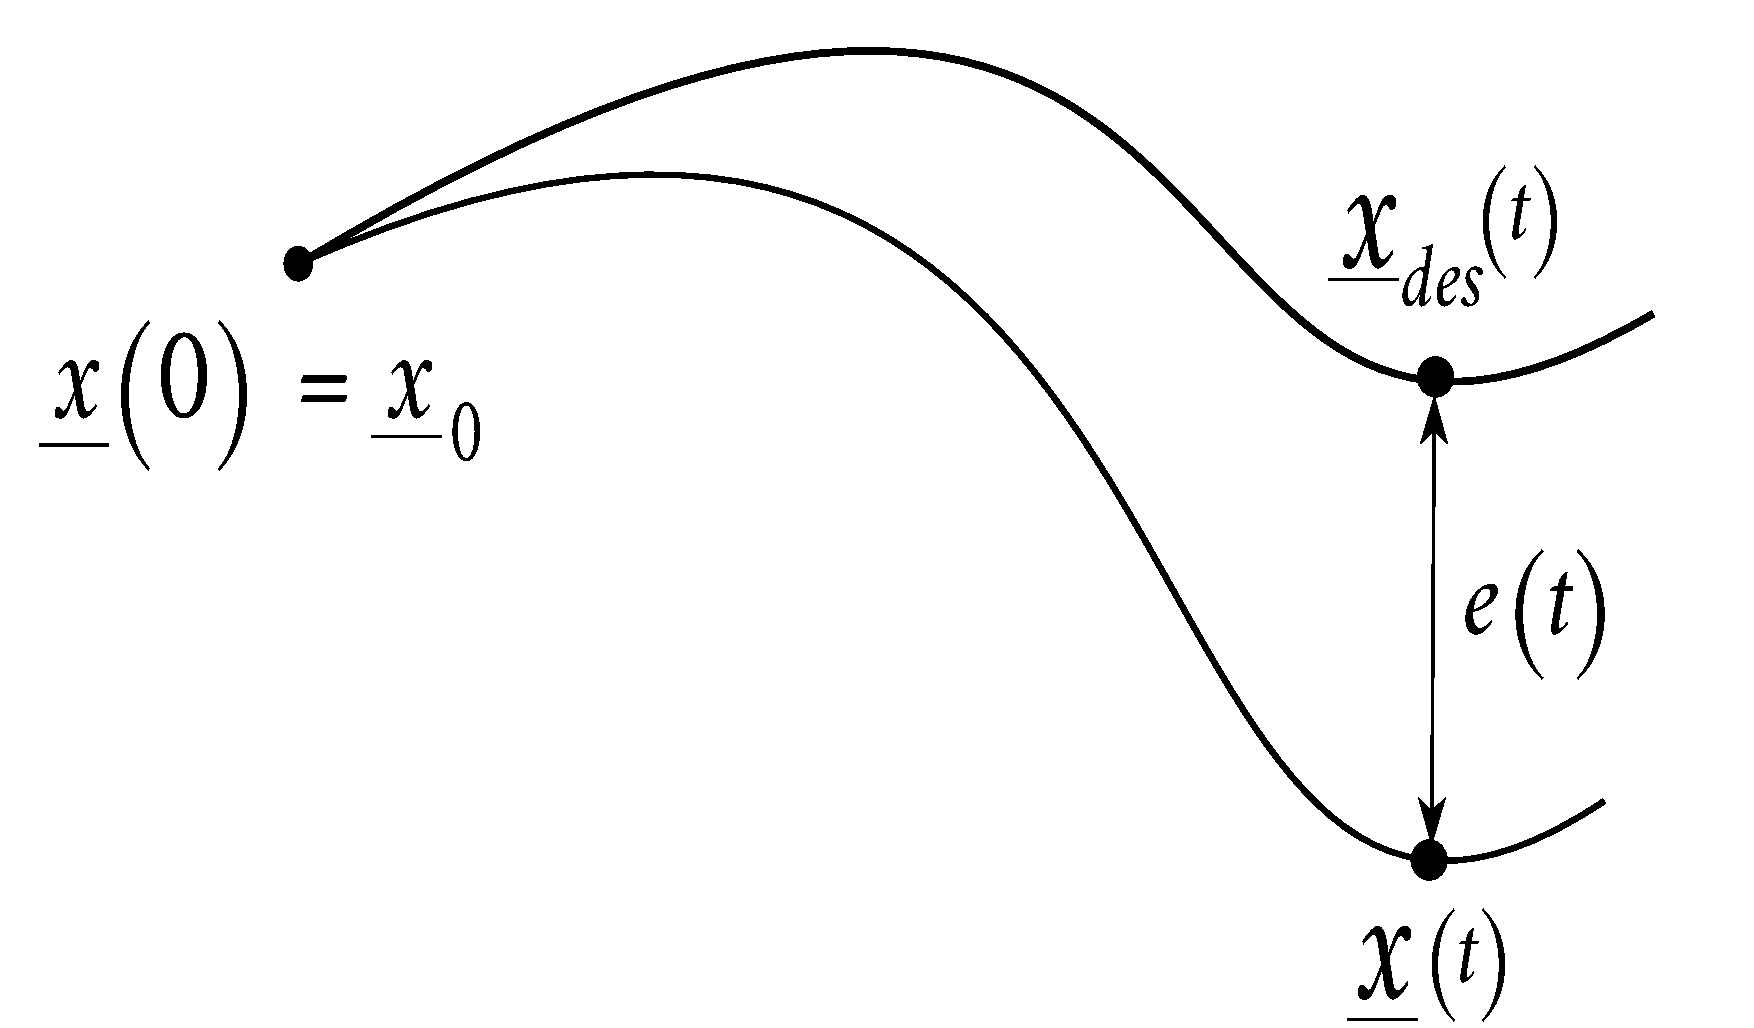
\includegraphics[scale=0.15]{errore.pdf}
\end{center}
Consideriamo la derivata temporale dell'errore che considerando la ($4.6$) otteniamo,
\begin{equation}
	\underline{\dot{e}} = \underline{\dot{x}}_{\,des} - \underline{\dot{x}} = \underline{\dot{x}}_{\,des} - J_a(\underline{q})\underline{\dot{q}}
\end{equation}
per far si che l'equazione ($5.19$) dia luogo ad un \emph{algoritmo per l'inversione cinematica}, servono due condizioni:
\begin{enumerate}
	\item La dipendenza tra $\underline{\dot{q}}$ ed $\underline{e}$ deve dare vita ad una equazione differenziale che caratterizzi l'evoluzione dell'errore nel tempo.
	\item La dipendenza tra $\underline{\dot{q}}$ ed $\underline{e}$ deve assicurare la convergenza a zero dell'errore.
\end{enumerate}
questa dipendenza da vita ai seguenti algoritmi \emph{closed loop inverse kinematic} (clik) per l'inversione cinematica. 

\subsection{Pseudo-inversa dello Jacobiano}
\paragraph{}
Ipotizziamo che la matrice $J_a$ quadrata sia \emph{non} singolare, possiamo scrivere $\underline{\dot{q}}$ in maniera algoritmica,
\begin{equation}
	\underline{\dot{q}} = J_a^{-1}(\underline{q})(\underline{\dot{x}}_{\,des} + K\underline{e})
\end{equation}
ottenendo 
\begin{equation}
	\underline{\dot{e}} + K\underline{e} = 0 \quad \Rightarrow \quad \underline{e}(t) = e^{-Kt}e_0,\;\; e_0 = 0
\end{equation}
se gli autovalori di $-K$ sono a parte reale negativa allora il sistema è globalmente e asintoticamente stabile. In effetti, la matrice $K$ è \emph{definita positiva} come scelta del progettista. 

Quindi l'errore tende a zero lungo la traiettoria con una velocità di convergenza che dipende dagli autovalori di $K$, più questi sono grandi, più veloce è la convergenza.

Lo schema a blocchi che realizza l'inversione cinematica secondo la ($5.20$) è rappresentato in Figura ($5.1$), 
\begin{center}
	\includegraphics[scale=0.35]{algInversaJacobiano.pdf}
	\caption{Schema a blocchi dell'algoritmo per l'inversione cinematica con $J_a^{-1}$}
\end{center}
analizziamolo:
\begin{itemize}
	\item Il blocco $K$ rappresenta un guadagno costante che rende il sistema asintoticamente stabile.
	\item Il blocco $kin(\cdot)$ rappresenta la funzione cinematica diretta, è un blocco non lineare ed è necessario al computo di $\underline{x}_{\,des}$ e anche al relativo errore di inseguimento.
	\item Il blocco $J_a^{-1}$ compensa $J_a$ e quindi fa si che il sistema sia lineare.
	\item Il blocco $\int$ nella catena diretta garantisce per un riferimento costante ($\underline{\dot{x}}_{\,des} = 0$) un errore a regime nullo.
	\item L'azione in \emph{feedforward} fornita da $\underline{\dot{x}}_{\,des}$ garantisce, in caso di riferimento non costante nel tempo, che l'errore si mantenga nullo lungo la traiettoria. Chiaramente, deve valere $\underline{e}(0) = 0$. 
\end{itemize}
\paragraph{}
Nel caso di un \emph{manipolatore ridondante}, la generalizzazione della ($5.20$) consente di ricavare una soluzione algoritmica del tipo,
\begin{equation}
	\underline{\dot{q}} = J^+_a(\underline{x}_{\,des} + K\underline{e}) + (I - J^+_aJ_a)\underline{\dot{q}}_{\,a}
\end{equation}
che corrisponde alla ($5.13$).

La struttura dell'algoritmo per l'inversione cinematica può essere concettualmente adottata ai fini di una tecnica di controllo semplice di un robot, nota sotto il nome di \emph{controllo cinematico}.

\subsection{Trasposta dello Jacobiano}
Un algoritmo di inversione cinematica più semplice di quello precedente dal punto di vista computazionale può essere ricavato dal legame tra $\underline{\dot{q}}$ ed $\underline{e}$ che assicuri la convergenza a zero dell'errore ma che non effettui la linearizzazione della ($5.19$). 

Quindi, la dinamica di errore è governata da un'equazione differenziale non lineare. Utilizziamo il \emph{metodo diretto di Lyapunov} per assicurarci la stabilità del sistema. I passi da seguire sono:
\begin{itemize}
	\item Definiamo una funzione candidata di Lyapunov $V(\underline{e})>0$ \emph{radially unbounded}.
	\item Cerchiamo $\underline{\dot{q}}$ in modo che $\dot{V}(\underline{e}) \leqslant 0$
\end{itemize}
\paragraph{}
Si scelga come funzione cadidata di Lyapunov la forma quadratica definita positiva
\begin{equation}
	V(\underline{e}) = \frac{1}{2}\underline{e}^TK\underline{e}
\end{equation} 
con $K$ matrice simmetrica e definita positiva. Tale funzione gode della seguente proprietà
\begin{equation}
	V(\underline{e})>0\quad \forall \underline{e} \neq \underline{0}, \quad V(\underline{0})= 0
\end{equation}
e pertanto differenziando la ($5.23$) rispetto al tempo e considerando la ($5.19$), si ha
\begin{equation}
	\dot{V}(\underline{e}) = \frac{\partial V}{\partial \underline{e}}\, \underline{\dot{e}} = \underline{e}^T K \underline{\dot{e}} = \underline{e}^TK \underline{\dot{x}}_{\,des} - \underline{e}^TK \underline{\dot{x}}
\end{equation}
A questo punto, scegliendo la velocità ai giunti come,
\begin{equation}
	\underline{\dot{q}} = J_a^TK\underline{e}
\end{equation}
otteniamo,
\begin{equation}
	\dot{V}(\underline{e}) = \underline{e}^TK \underline{\dot{x}}_{\,des} - \underline{e}^TK J_aJ_a^TK\underline{e}
\end{equation}
\paragraph{}
Si consideri il caso di riferimento costante, ovvero $\underline{\dot{x}}_{\,des} = \underline{0}$, otteniamo
\begin{equation}
	\dot{V}(\underline{e}) = - \underline{e}^TK J_aJ_a^TK\underline{e}
\end{equation}

notiamo che:
\begin{itemize}
	\item Se ipotizziamo che $J_a$ sia di rango pieno, la funzione ($5.28$) risulta \emph{definita negativa}.
	\item Se inoltre, imponiamo $\dot{V}<0$ e $V>0$ otteniamo $\underline{e} = \underline{0}$, ovvero, il sistema risulta \emph{asintoticamente stabile}.
	\item Se $\mathcal{N}(J_a^T) \neq 0$, la funzione ($5.28$) risulta \emph{semi-definita negativa}, infatti otteniamo che $\dot{V} = 0$ per $\underline{e} \neq \underline{0}$ e pertanto $K\underline{e} \in \mathcal{N}(J_a^T)$. In questo caso la ($5.28$) evidenzia che l'algoritmo si trova in \emph{stallo}, ovvero, $\underline{\dot{q}} = \underline{0}$, ottenendo \emph{stabilità marginale}. In realtà, questa situazione si presenta solo se la posa assegnata dell'organo terminale, effettivamente non è raggiungibile dalla configurazione corrente.  
\end{itemize} 
\paragraph{}
Lo schema a blocchi dell'inversione cinematica è rappresentato di seguito,
\begin{center}
	\includegraphics[scale=0.35]{algTraspostaJacobiano.pdf}
	\caption{Schema a blocchi dell'algoritmo per l'inversione cinematica con $J_a^T$}
\end{center}
analizziamo che la caratteristica notevole dell'algoritmo è quella di richiedere il funzionamento di sole funzioni cinematiche dirette, $kin(\cdot)$, $J_a^T(\cdot)$.

Notiamo che se $\underline{\dot{x}}_{\,des} \neq \underline{0}$, il termine a primo membro della ($5.27$) non viene cancellato e nulla si può dire sul segno del secondo membro. Ciò comporta che non è possibile ottenere \emph{l'asintotica stabilità} lungo la traiettoria. L'errore di inseguimento è comunque limitato superiormente.

In definitiva, l'algoritmo basato sul calcolo della trasposta dello Jacobiano fornisce un metodo di inversione cinematica efficiente da un punto di vista computazionale che può essere utilizzato anche nel caso di percorsi passanti per singolarità cinematiche.
\subsubsection{Esempio manipolatore 2R}
Con riferimento alla seguente figura,
\begin{center}
	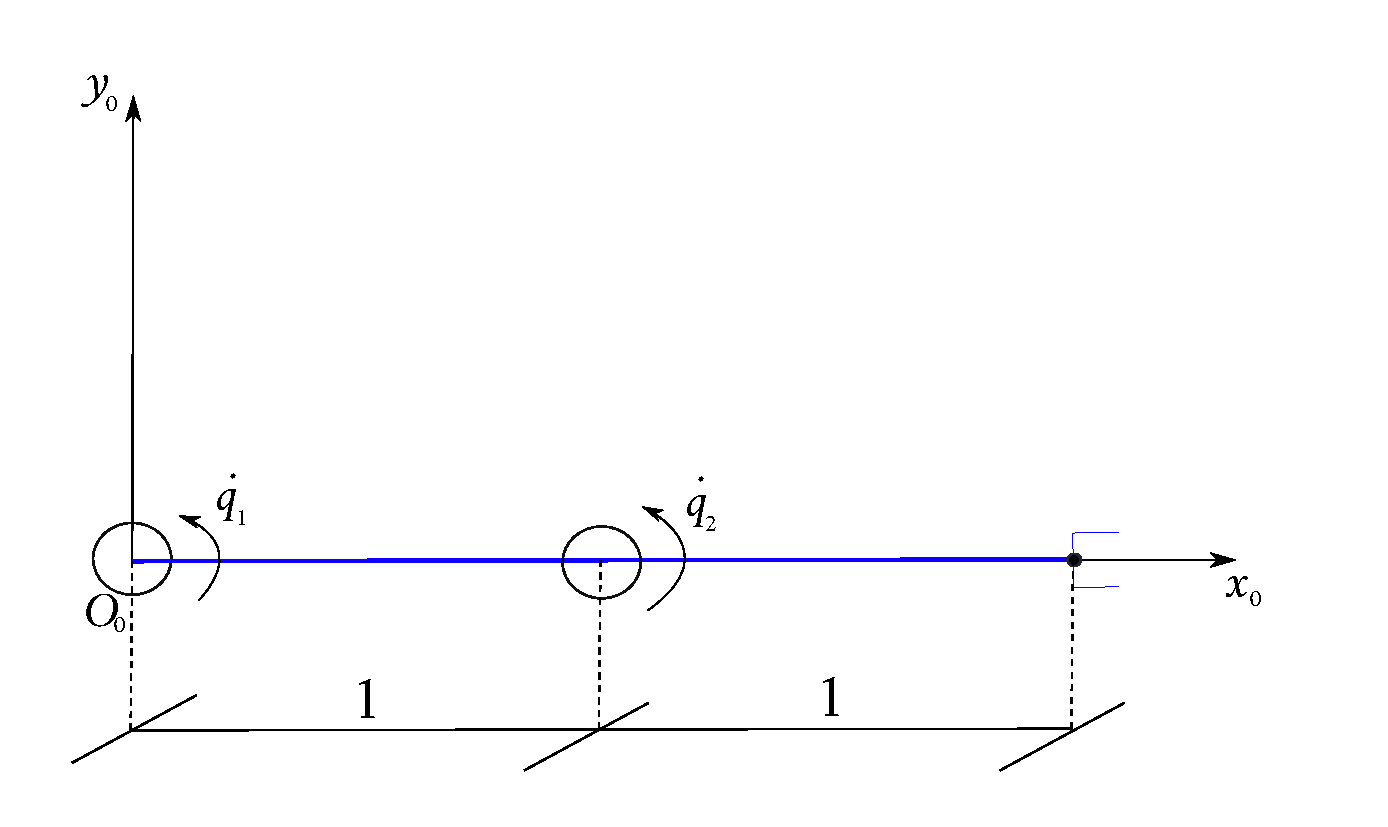
\includegraphics[scale=0.3]{manipolatoreStallo2R.pdf}
\end{center}
otteniamo
\begin{equation}
	\begin{bmatrix}
		\dot{x} \\
		\dot{y} \\
	\end{bmatrix}
	= 
	\underbrace{
	\begin{bmatrix}
		0 & 0 \\
		2 & 1 \\
	\end{bmatrix}
	}_{J_a}
	\begin{bmatrix}
		\dot{q}_1 \\
		\dot{q}_2 \\
	\end{bmatrix}
\end{equation}
calcoliamo $\mathcal{R}(J_a)$ e $\mathcal{N}(J_a^T)$,
\begin{equation}
	J_a = 
	\begin{bmatrix}
		0 & 0 \\
		2 & 1 \\
	\end{bmatrix}
	\; \Rightarrow \; \mathcal{R}(J_a) = 
	\begin{bmatrix}
		0 \\
		1 \\
	\end{bmatrix}
	\qquad 
	J_a^T = 
	\begin{bmatrix}
		0 & 2 \\
		0 & 1 \\
	\end{bmatrix}
	\; \Rightarrow \; \mathcal{N}(J_a^T) = 
	\begin{bmatrix}
		1 \\
		0 \\
	\end{bmatrix}
\end{equation}
distinguiamo due casi: il caso in cui il sistema va in stallo e quello in cui non va in stallo,
\begin{itemize}
	\item Ipotizziamo, 
	\begin{equation*}
		K =
		\begin{bmatrix}
			1 & 0 \\
			0 & 1 \\
		\end{bmatrix}
		, \qquad \underline{x}_{\,des} =  
		\begin{bmatrix}
			2 \\
			\varepsilon \\
		\end{bmatrix}
		, \qquad \underline{x} = 
		\begin{bmatrix}
			2 \\
			0 \\
		\end{bmatrix}
	\end{equation*}
	otteniamo 
	\begin{equation*}
		K \underline{e} = 
		\begin{bmatrix}
			1 & 0 \\
			0 & 1 \\
		\end{bmatrix}
		\begin{bmatrix}
			0 \\
			\varepsilon \\
		\end{bmatrix}
		=
		\begin{bmatrix}
			0 \\
			\varepsilon \\
		\end{bmatrix}
		\not\in\mathcal{N}(J_a^T)
	\end{equation*}
	in questo caso il sistema \emph{non} va in stallo.
	
	\item Cerchiamo una $\underline{x}_{\,des}$ che manda in \emph{stallo} il sistema, ovvero
	\begin{equation*}
		\underline{x}_{\,des} =
		\begin{bmatrix}
			2+\varepsilon \\
			0 \\
		\end{bmatrix},
		\qquad 
		\underline{x}_{\,des} =
		\begin{bmatrix}
			2-\varepsilon \\
			0 \\
		\end{bmatrix}
	\end{equation*}
	mandano in stallo il sistema, infatti
	\begin{equation*}
		K \underline{e} = 
		\begin{bmatrix}
			1 & 0 \\
			0 & 1 \\
		\end{bmatrix}
		\begin{bmatrix}
			\varepsilon \\
			0 \\
		\end{bmatrix}
		=
		\begin{bmatrix}
			\varepsilon \\
			0 \\
		\end{bmatrix}
		\in\mathcal{N}(J_a^T)
	\end{equation*}
\end{itemize}

\subsubsection{Interpretazione fisica}
Notiamo una interessante interpretazione fisica di questo algoritmo, tale interpretazione userà nozioni di statica spiegate in seguito. 

Supponendo che il manipolatore sia caratterizzato da una dinamica ideale $\underline{\tau} = \underline{\dot{q}}$ (masse nulle e coefficienti di attrito viscoso unitari), lo schema di inversione svolge la funzione di una \emph{molla generalizzata}, di costante $K$, che genera una forza $K \underline{e}$ che tira l'organo terminale verso la posa desiderata nello spazio operativo.

Se a tale manipolatore è concesso di muoversi, e ciò è possibile solo se $K\underline{e} \not \in \mathcal{N}(J^T)$, l'organo terminale assume la posa desiderata e possono essere individuate le variabili corrispondenti nello spazio dei giunti.

\subsection{Errore di orientamento}
Abbiamo notato che gli algoritmi per l'inversione cinematica operano su \emph{variabili di errore} che sono definite nello spazio operativo. L'errore è di tipo \emph{posizionale} o di \emph{orientamento}. Per quanto riguarda l'errore posizionale, la sua espressione è data da
\begin{equation}
	\underline{e}_{\,p} = \underline{p}_{\,d} - \underline{p}
\end{equation} 
dove $\underline{p}_{\,d}$ e $\underline{p}$ denotano rispettivamente \emph{posizione desiderata} e \emph{posizione dell'organo terminale}. La sua derivata è
\begin{equation}
	\underline{\dot{e}}_{\,p} = \underline{\dot{p}}_{\,d} - \underline{\dot{p}}
\end{equation}

\paragraph{}
Per quanto riguarda \emph{l'errore di orientamento}, la sua espressione dipende dalla rappresentazione dell'organo terminale. Scegliamo la \emph{rappresentazione Asse-Angolo}.

Indicando con  
$R_d = 
\begin{bmatrix}
	\underline{n}_d & \underline{s}_d & \underline{a}_d
\end{bmatrix}$ la matrice di rotazione della terna utensile di riferimento e con 
$R =
\begin{bmatrix}
	\underline{n} & \underline{s} & \underline{a}
\end{bmatrix}$ quella della terna utensile relativa alle variabili di giunto effettive. 

L'errore di orientamento tra le due terne può essere espresso come
\begin{equation}
	\underline{e}_{\,o} = \underline{r}\sin\vartheta
\end{equation}
dove $\underline{r}$ e $\vartheta$ caratterizzano \emph{l'asse e l'angolo} di rotazione. Sviluppando si ottiene,
\begin{equation}
	\underline{e}_{\,o} = \frac{1}{2}
	\begin{bmatrix}
		\underline{n} \times \underline{n}_{\,d} + \underline{s} \times \underline{s}_{\,d} + \underline{a} \times \underline{a}_{\,d}
	\end{bmatrix}
\end{equation}
e derivando tenendo conto di $\dot{R}(t) = S(t)R(t)$, otteniamo
\begin{equation}
	\underline{\dot{e}}_{\,o} = L^T\underline{\omega}_{\,d} - L\underline{\omega}
\end{equation}
con $L \in \mathbb{R}^{3 \times 3}$ invertibile.

\paragraph{}
Adesso studiamo la dinamica dell'errore \emph{complessiva}, 
\begin{equation*}
	\underline{\dot{e}} = 
	\begin{bmatrix}
		\underline{\dot{e}}_{\,p} \\
		\underline{\dot{e}}_{\,o} \\
	\end{bmatrix}
	=
	\begin{bmatrix}
		\underline{\dot{p}}_{\,d} - \underline{\dot{p}} \\
		L^T \underline{\omega}_{\,d} - L \underline{\omega} \\
	\end{bmatrix}
	= 
	\begin{bmatrix}
		\underline{\dot{p}}_{\,d} - J_p\underline{\dot{q}} \\
		L^T\underline{\omega}_{\,d} - LJ_o\underline{\dot{q}} \\
	\end{bmatrix}
	=
\end{equation*}
\begin{equation}
	=
	\begin{bmatrix}
		\underline{\dot{p}}_{\,d} \\
		L^T \underline{\omega}_{\,d} \\
	\end{bmatrix}
	-
	\begin{bmatrix}
		J_p\underline{\dot{q}} \\
		LJ_o\underline{\dot{q}} \\
	\end{bmatrix}
	 = 
	 \begin{bmatrix}
	 	\underline{\dot{p}}_{\,d} \\
		L^T \underline{\omega}_{\,d} \\
	 \end{bmatrix}
	 -
	 \begin{bmatrix}
	 	I & 0 \\
	 	0 & L \\
	 \end{bmatrix}
	 \underbrace{
	 \begin{bmatrix}
	 	J_p \\
	 	J_o \\
	 \end{bmatrix}
	 }_{J}
	 \underline{\dot{q}}
\end{equation}
e considerando che vogliamo un sistema asintoticamente stabile nell'origine, vogliamo che $\underline{\dot{e}}$ sia uguale ad una matrice con autovalori a parte reale negativa moltiplicata l'errore $\underline{e}$. 

Quindi, otteniamo l'espressione $\underline{\dot{e}} + K \underline{e} = \underline{0}$ seguente
\begin{equation*}
	\underline{\dot{e}} + K \underline{e} = 
	\begin{bmatrix}
		\underline{\dot{e}}_{\,p} \\
		\underline{\dot{e}}_{\,o} \\
	\end{bmatrix}
	+
	\begin{bmatrix}
		K_p & 0 \\
		0 & K_o \\
	\end{bmatrix}
	\begin{bmatrix}
		\underline{e}_{\,p} \\
		\underline{e}_{\,o} \\
	\end{bmatrix}
	=
\end{equation*}
\begin{equation}
	=
	\begin{bmatrix}
	 	\underline{\dot{p}}_{\,d} \\
		L^T \underline{\omega}_{\,d} \\
	\end{bmatrix}
	-
	\begin{bmatrix}
	 	I & 0 \\
	 	0 & L \\
	\end{bmatrix}
	J
	\underline{\dot{q}}
	+ 
	\begin{bmatrix}
		K_p \underline{e}_{\,p} \\
		K_o \underline{e}_{\,o} \\
	\end{bmatrix}
	= 
	\begin{bmatrix}
		0 \\
		0 \\
	\end{bmatrix}
\end{equation}
per analogia agli algoritmi di inversione visti fino ad ora, il legame tra $\underline{\dot{q}}$ ed $\underline{e}$ è ottenuto mediante l'inversione dello \emph{Jacobiano Geometrico} in luogo di quello \emph{Analitico}.

Calcoliamo la soluzione con inversa dello Jacobiano,
\begin{equation*}
	-
	\begin{bmatrix}
		I & 0 \\
		0 & L \\
	\end{bmatrix}
	J \underline{\dot{q}} =
	- 
	\begin{bmatrix}
		\underline{\dot{p}}_{\,d} \\
		L^T \underline{\omega}_{\,d} \\
	\end{bmatrix}	
	-
	\begin{bmatrix}
		K_p \underline{e}_{\,p} \\
		K_o \underline{e}_{\,o} \\
	\end{bmatrix}
	\quad \Rightarrow \quad
	\begin{bmatrix}
		I & 0 \\
		0 & L \\
	\end{bmatrix}
	J \underline{\dot{q}} =
	\begin{bmatrix}
		\underline{\dot{p}}_{\,d} + K_p \underline{e}_{\,p} \\
		L^T \underline{\omega}_{\,d} + K_o \underline{e}_{\,o} \\
	\end{bmatrix}
	\quad \Rightarrow
\end{equation*}
\begin{equation*}
	\Rightarrow \quad 
	J \underline{\dot{q}} = 
	\begin{bmatrix}
		I & 0 \\
		0 & L^{-1} \\
	\end{bmatrix}
	\begin{bmatrix}
		\underline{\dot{p}}_{\,d} + K_p \underline{e}_{\,p} \\
		L^T \underline{\omega}_{\,d} + K_o \underline{e}_{\,o} \\
	\end{bmatrix}
\end{equation*}
e otteniamo la soluzione per un manipolatore non ridondante e non in singolarità,
\begin{equation}
	\underline{\dot{q}} = J^{-1}
	\begin{bmatrix}
		\underline{\dot{p}}_{\,d} + K_p \underline{e}_{\,p} \\
		L^{-1}(L^T \underline{\omega}_{\,d} + K_o \underline{e}_{\,o}) \\
	\end{bmatrix}
\end{equation}
osserviamo che questa soluzione della cinematica inversa offre migliore prestazioni perchè impiegando lo Jacobiano Geometrico, si evitano l'insorgere di singolarità di rappresentazione.

Per gestire esplicitamente la \emph{singolarità} possiamo usare la \emph{pseudo-inversa smorzata} $J^*$ definita dalla ($5.15$), ottenendo la seguente soluzione,
\begin{equation}
	\underline{\dot{q}} = \underbrace{J^T(JJ^T + K^2I)^{-1}}_{J^*}  
	\begin{bmatrix}
		\underline{\dot{p}}_{\,d} + K_p \underline{e}_{\,p} \\
		L^{-1}(L^T \underline{\omega}_{\,d} + K_o \underline{e}_{\,o}) \\
	\end{bmatrix}
\end{equation}